\documentclass[twoside]{article}

\usepackage{aistats2023}
\usepackage{amsmath}
\usepackage{amssymb}
\newtheorem{theorem}{Theorem}[section]
\newtheorem{corollary}{Corollary}[theorem]
\DeclareMathOperator*{\argmin}{arg\,min}

\usepackage{graphicx}
\graphicspath{ {./../examples/} }


\newcommand{\dfdx}{\frac{\partial f}{\partial x_s}}
\newcommand{\xc}{\mathbf{x_c}}
\newcommand{\DY}{\mathbf{\Delta Y}}
\newcommand{\xb}{\mathbf{x}}
\newcommand{\Xcb}{\mathcal{X}_c}
\newcommand{\Xb}{\mathcal{X}}

% If your paper is accepted, change the options for the package
% aistats2022 as follows:
%
%\usepackage[accepted]{aistats2022}
%
% This option will print headings for the title of your paper and
% headings for the authors names, plus a copyright note at the end of
% the first column of the first page.

% If you set papersize explicitly, activate the following three lines:
%\special{papersize = 8.5in, 11in}
%\setlength{\pdfpageheight}{11in}
%\setlength{\pdfpagewidth}{8.5in}

% If you use natbib package, activate the following three lines:
%\usepackage[round]{natbib}
%\renewcommand{\bibname}{References}
%\renewcommand{\bibsection}{\subsubsection*{\bibname}}

% If you use BibTeX in apalike style, activate the following line:
%\bibliographystyle{apalike}

\begin{document}

% If your paper is accepted and the title of your paper is very long,
% the style will print as headings an error message. Use the following
% command to supply a shorter title of your paper so that it can be
% used as headings.
%
%\runningtitle{I use this title instead because the last one was very long}

% If your paper is accepted and the number of authors is large, the
% style will print as headings an error message. Use the following
% command to supply a shorter version of the authors names so that
% they can be used as headings (for example, use only the surnames)
%
%\runningauthor{Surname 1, Surname 2, Surname 3, ...., Surname n}

% Supplementary material: To improve readability, you must use a single-column format for the supplementary material.
\onecolumn
\aistatstitle{Instructions for Paper Submissions to AISTATS 2023: \\
Supplementary Materials}

\section{THORETICAL DERIVATIONS}

\subsection{Show that \(\hat{\mu}(z_1, z_2) \approx \mu(z_1, z_2)\)}

\textit{We want to show that (a)
  \(\hat{\mu}(z_1, z_2) = \frac{1}{|\mathcal{S}|} \sum_{i:
    \mathbf{x}^i \in \mathcal{S}} f^s(\mathbf{x}^i) \) is an unbiased
  estimator of
  \(\mu(z_1, z_2) = \frac{\int_{z_1}^{z_2} \mathbb{E}_{X_c|z} \left [
      f^s(z, X_c) \right ] \partial z}{z_2 - z_1} \), under the
  assumption that that (a) \(z\) follows a uniform distribution in
  \([z_1, z_2)\), i.e., \(z \sim \mathcal{U}(z_1, z_2)\) and (b) that
  the points are i.i.d.  samples from the distribution
  \(p(\xb) = p(\xc|z)p(z) = \frac{1}{z_2-z_1}p(\xc|z) \) }

\paragraph{Description}
  We just use the the fact that the population mean is an
  unbiased estimator of the expected value. We just show that
  \(\mu(z_1, z_2) = \mathbb{E}_{\tilde{X}} [f^s(\tilde{X})]\).

\paragraph{Proof}
\begin{align}
  \mu(z_1, z_2) = \frac{\int_{z_1}^{z_2} \mathbb{E}_{X_c|z} f^s(z, X_c)  \partial z}{z_2 - z_1}
                = \mathbb{E}_{z \sim \mathcal{U}(z_1, z_2)}\mathbb{E}_{X_c|z} f^s(z, X_c)
                = \mathbb{E}_{\tilde{X}} f^s(X)
\end{align}

\subsection{Show that \(\hat{\sigma}^2(z_1, z_2) \approx  \sigma_*^2(z_1, z_2)\)}

\textit{We want to show that \(\hat{\sigma}^2(z_1, z_2) = \frac{1}{|\mathcal{S}_k|}
\sum_{i:\mathbf{x}^i \in \mathcal{S}_k} \left ( \dfdx(\mathbf{x}^i) -
  \hat{\mu}(z_1, z_2) \right )^2\) is an unbiased
estimator of
\(\sigma^2_*(z_1, z_2) = \frac{\int_{z_1}^{z_2} \mathbb{E}_{X_c|X_s=z}
  \left [ (f^s(z, X_c) - \mu(z_1, z_2) )^2 \right] \partial z}{z_2 -
  z_1} \), , under the
  assumption that that (a) \(z\) follows a uniform distribution in
  \([z_1, z_2)\), i.e., \(z \sim \mathcal{U}(z_1, z_2)\) and (b) that
  the points are i.i.d.  samples from the distribution
  \(p(\xb) = p(\xc|z)p(z) = \frac{1}{z_2-z_1}p(\xc|z) \).}

\paragraph{Description}
Same as before, we just use the the fact that the population variance
is an unbiased estimator of the variance. We just show that
\(\sigma^2_*(z_1, z_2) = \mathbb{V}_{\tilde{X}} [f^s(\tilde{X})]\).

\paragraph{Proof}


\begin{align}
  \sigma^2_*(z_1, z_2) & = \frac{\int_{z_1}^{z_2} \mathbb{E}_{X_c|X_s=z}
                         \left [ (f^s(z, X_c) - \mu(z_1, z_2) )^2 \right] \partial z}{z_2 -
                         z_1} \\
                       & = \mathbb{E}_{z \sim \mathcal{U}(z_1, z_2)}\mathbb{E}_{X_c|X_s=z}
                         \left [ (f^s(z, X_c) - \mu(z_1, z_2) )^2 \right] \\
                       & = \mathbb{E}_{\tilde{X}} \left [ (f^s(X) - \mu(z_1, z_2) )^2 \right]\\
                       & = \mathbb{V}_{\tilde{X}} [f^s(\tilde{X})]
  \end{align}


\subsection{Proof Of Theorem 3.1}

\textit{If we define (a) the residual \(\rho(z)\) as the difference between
  the expected effect at \(z\) and the bin-effect, i.e
  \(\rho(z) = \mu(z) - \mu(z_1, z_2)\) and (b)
  \(\mathcal{E}(z_1, z_2)\) as the mean squared residual of the bin,
  i.e.
  \(\mathcal{E}(z_1, z_2) = \frac{\int_{z_1}^{z_2}\rho^2(z) \partial
    z}{z_2 - z_1}\), then it holds that:
\begin{equation}
    \label{eq:bin-uncertainty-proof}
 \sigma_*^2(z_1, z_2) = \sigma^2(z_1, z_2) + \mathcal{E}^2(z_1, z_2)
\end{equation}
}


\paragraph{Proof}


\begin{align}
  \sigma_*^2(z_1, z_2) &= \frac{1}{z_2 - z_1}\int_{z_1}^{z_2} \mathbb{E}_{X_c|z} \left [ \left( f^s( z, X_c) - \mu(z_1, z_2) \right)^2 \right] \partial z \\
                       &= \frac{1}{z_2 - z_1} \int_{z_1}^{z_2} \mathbb{E}_{X_c|z} \left [ \left ( f^s(z, X_c) - \mu(z) + \rho(z) \right )^2 \right] \partial z \\
  &= \frac{1}{z_2 - z_1} \int_{z_1}^{z_2} \mathbb{E}_{X_c|z} \left [ (f^s(z, X_c) - \mu(z) )^2 + \rho(z)^2 + 2f^s(z, X_c)\mu(z) ) \right ]\\
  &= \frac{1}{z_2 - z_1} \int_{z_1}^{z_2} \left (
  \underbrace{\mathbb{E}_{X_c|z} \left [ (f^s(z, X_c) - \mu(z) )^2 \right ]}_{\sigma^2(z)}  +
  \underbrace{\mathbb{E}_{X_c|z} \left [ \rho^2(z) \right]}_{\rho^2(z)} +
  2 (\underbrace{\mathbb{E}_{X_c|z} \left [ (f^s(z, X_c)   \right ]}_{\mu(z)} - \mu(z)) \rho(z) )\right )  \partial z \\
  &= \underbrace{\frac{1}{z_2 - z_1} \int_{z_1}^{z_2} \sigma^2(z) \partial z}_{\sigma^2(z_1, z_2)} + \underbrace{\frac{1}{z_2 - z_1} \int_{z_1}^{z_2} \rho^2(z) \partial z}_{\mathcal{E}^2(z_1, z_2)} = \sigma^2(z_1, z_2) + \mathcal{E}^2(z_1, z_2)
\end{align}

\subsection{Proof Of Corollary}

\textit{ If a bin-splitting \(\mathcal{Z}\) minimizes the accumulated error, then it also minimizes
  \(\sum_{k=1}^K\sigma_*^2(z_1, z_2) \Delta z_k \)}

We want to show that

\[ \mathcal{Z}^* = \argmin_{\mathcal{Z}} \sum_{k=1}^K \sigma_*^2(z_{k-1}, z_k) \Delta z_k \Leftrightarrow \mathcal{Z}^* = \argmin_{\mathcal{Z}} \sum_{k=1}^K \mathcal{E}^2(z_{k-1}, z_k) \Delta z_k \]

\paragraph{Proof}

\begin{align}
  \mathcal{Z}^* &= \argmin_{\mathcal{Z}} \sum_{k=1}^K \sigma_*^2(z_{k-1}, z_k) \Delta z_k \\
                & = \argmin_{\mathcal{Z}} \left [ \sum_{k=1}^K (\sigma^2(z_{k-1}, z_k) + \mathcal{E}^2(z_{k-1}, z_k)) \Delta z_k \right ] \\
                & = \argmin_{\mathcal{Z}} \left [ \sum_{k=1}^K \left ( \frac{\Delta z_k}{\Delta z_k} \int_{z_{k-1}}^{z_k} \sigma^2(z) \partial z)   + \mathcal{E}^2(z_{k-1}, z_k) \Delta z_k \right ) \right ] \\
                & = \argmin_{\mathcal{Z}} \left [ \underbrace{\int_{z_0}^{z_K} \sigma^2(z) \partial z}_{\text{independent of } \mathcal{Z}}   + \sum_{k=1}^K\mathcal{E}^2(z_{k-1}, z_k) \Delta z_k) \right ] \\
                & = \argmin_{\mathcal{Z}} \sum_{k=1}^K\mathcal{E}^2(z_{k-1}, z_k) \Delta z_k
  \end{align}

\section{Dynamic Programming Analysis}
\label{sec:dynamic-programming}

For achieving a computationally-grounded solution we set a threshold
\(K_{max}\) on the maximum number of bins which also discretizes the
solution space. The width of the bin can take discrete values that are
multiple of the minimum step
\(u = \frac{x_{s, max} - x_{s, min}}{K_{max}}\). For defining the
solution, we use two indexes. The index
\(i \in \{0, \ldots, K_{max}\}\) denotes the point \((z_i)\) and the
index \(j \in \{0, \ldots, K_{max}\} \) denotes the position of the
\(j\)-th multiple of the minimum step, i.e.,
\(x_j = x_{s,min} + j \cdot u\). The recursive cost function
\(T(i,j)\) is the cost of setting \(z_i=x_j\):
\begin{equation}
  \label{eq:recursive_cost}
  \mathcal{T}(i,j) = \mathrm{min}_{l \in \{0, \ldots, K_{max}\}} \left [ \mathcal{T}(i-1, l) + \mathcal{B}(x_l, x_j) \right ]
\end{equation}
%
where \(\mathcal{T}(0,j)\) equals zero if \(j=0\) and \(\infty\) in
any other case. \(\mathcal{B}(x_l, x_j)\) denotes the cost of creating a bin
with limits \([x_l, x_j)]\):

\begin{equation}
  \label{eq:cost_step}
  \mathcal{B}(x_l, x_j) = \begin{cases}
                            \infty, & \text{if $x_j > x_l$ or \(|\mathcal{S}_{(x_j, x_l)}| < N\)}\\
                            0, & \text{if $x_j = x_l$}\\
                            \hat{\sigma}^2(x_j, x_l), &\text{if $x_j \leq x_l$}
  \end{cases}
\end{equation}

The optimal solution is given by solving
\(\mathcal{L} = \mathcal{T}(K_{max}, K_{max})\) and keeping track of the sequence of
steps.


\section{Real World Experiment}

In this section, we provide further details on the real-world
example. The real-world example uses the California Housing Dataset,
which contains 8 numerical features. We exclude instances with missing
or outlier values. If we denote as \(\mu_s\) (\(\sigma_s\)) the
average value (standard deviation) of the \(s\)-th feature, we
consider outliers the instances of the training set with any feature
value over three standard deviations from the mean, i.e.
\(|x_s^i - \mu_s| > \sigma_s\). This preprocessing step discards
\(884\) instancies, and \(N=19549\) remain. We provide their
description with some basic descriptive statistics in
Table~\ref{tab:features-description} and their histogram in
Figure~\ref{fig:feature-histograms}.

In Figure 7 of the main paper, we provided the UALE vs PDP-ICE plots
for features \(x_2\) (latitude), \(x_6\) (total number of people) and
\(x_8\) (median house value). In figure 8, we compared UALE with
fixed-size approximation, for the same features. In
Figure~\ref{fig:ex-real-1}, we provide the same information for the
rest of the features; \(x_1\) (longitude), \(x_3\) (median age of
houses), \(x_4\) (total number of rooms), \(x_5\) (total number of
bedrooms) and \(x_7\) (total number of households). The observation of
these feautures leads us to similar conclusion. First, UALE and
PDP-ICE plots compute similar effects and level of heterogeneity and
UALE's approximation is (almost) as good as the best fixed-size
approximation. More specifically, we observe that UALE's variable size
bin splitting correctly creates wide bins for features
\(x_3, x_4, x_5, x_7\), where the feature effect plot is (piecewise)
linear, while using narrow bins for feature \(x_2\) where the feature
effect is not linear.

\begin{table}
  \caption{Description of the features apparent in the California-Housing Dataset}
  \label{tab:features-description}
  \centering
  \begin{tabular}{ c|c|c|c|c|c| }
    \hline
    & Description & \(min\) & \(\max\) & \(\mu\) & \(\sigma\) \\
    \hline
    \(x_1\) & longitude & \(-124.35\) & \(-114.31\) & \(-119.58\) & \(2\) \\
    \(x_2\) & latitude  & \(32.54\) & \(41.95\) & \(35.65\) & \(2.14\) \\
    \(x_3\) & median age of houses & \(1\) & \(52\) & \(29.01\) & \(12.42\) \\
    \(x_4\) & total number of rooms & \(2\) & \(9179\) & \(2390.79\) & \(1433.83\) \\
    \(x_5\) & total number of bedrooms & \(2\) & \(1797\) & \(493.86\) & \(291\) \\
    \(x_6\) & total number of people & \(3\) & \(4818\) & \(1310.91\) & \(771.78\) \\
    \(x_7\) & total number of households & \(2\) & \(1644\) & \(460.3\) & \(267.34\) \\
    \(x_8\) & median income of households & \(0.5\) & \(9.56\) & \(3.72\) & \(1.60\) \\
    \hline
    \(y\) & median house value & \(14.999\) & \(500000\) & \(206864.41\) & \(115435.67\) \\
    \hline
  \end{tabular}
\end{table}


\begin{figure}[h]
  \centering
  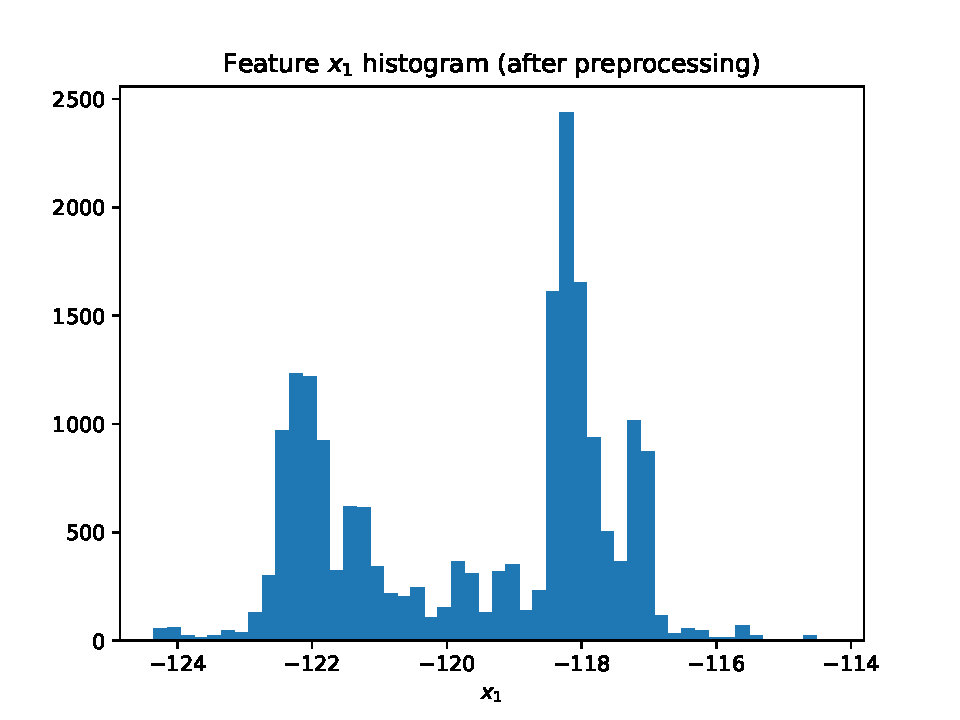
\includegraphics[width=.43\textwidth]{real_dataset_3/hist_feat_1_after.pdf}
  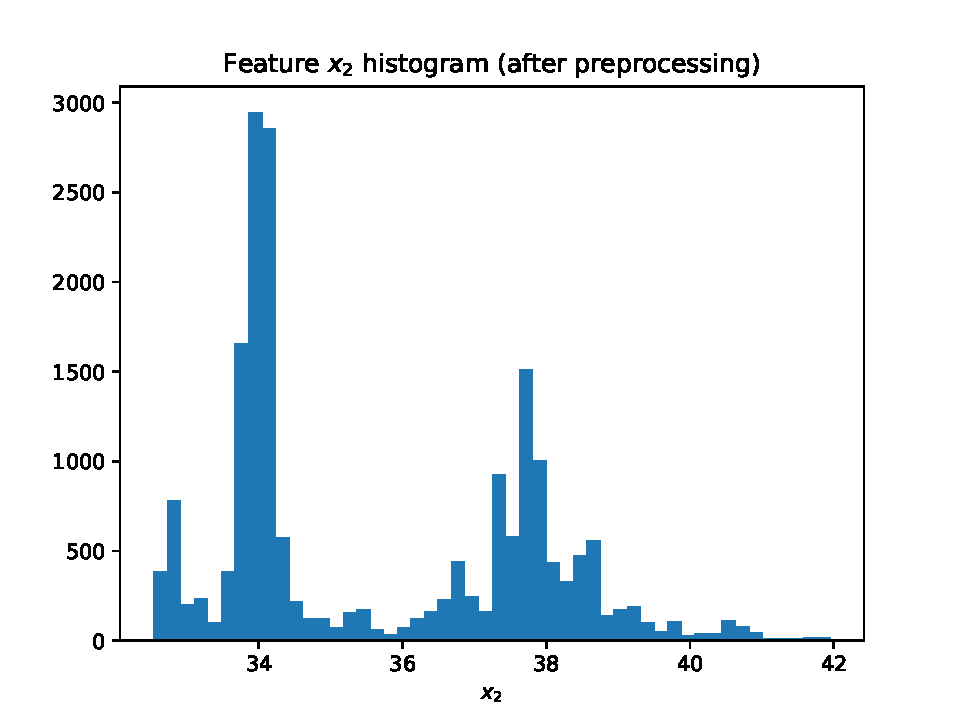
\includegraphics[width=.43\textwidth]{real_dataset_3/hist_feat_2_after.pdf}\\
  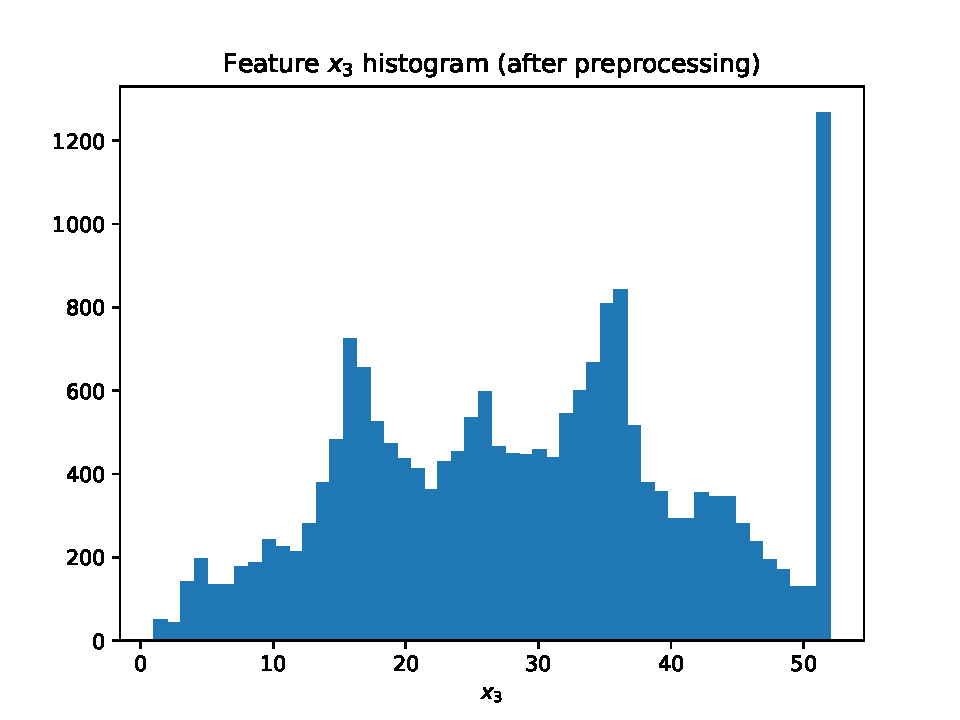
\includegraphics[width=.43\textwidth]{real_dataset_3/hist_feat_3_after.pdf}
  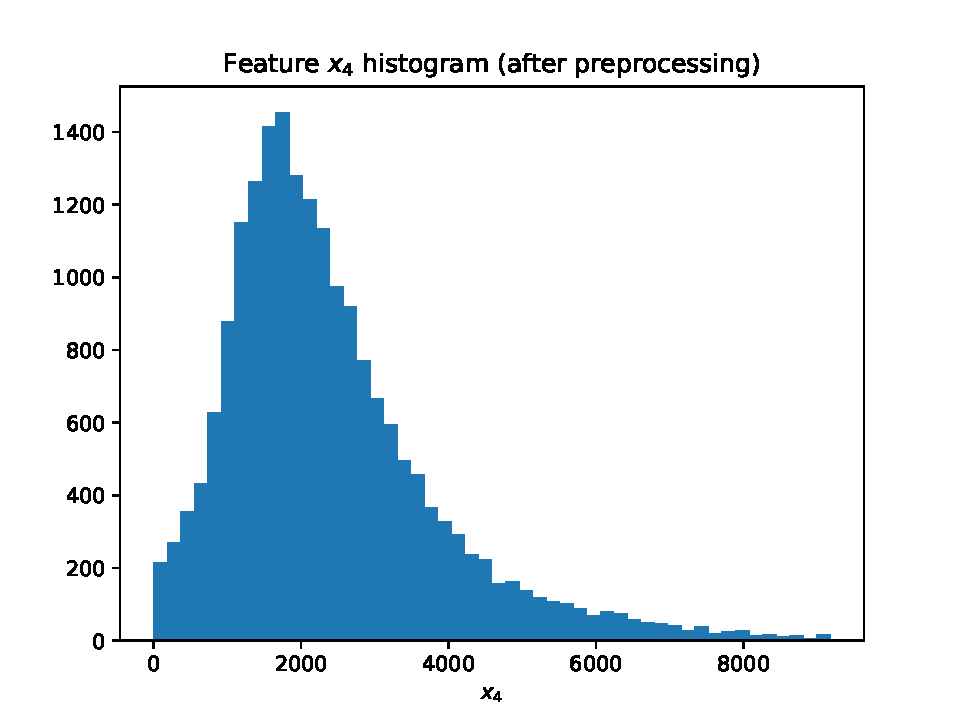
\includegraphics[width=.43\textwidth]{real_dataset_3/hist_feat_4_after.pdf}\\
  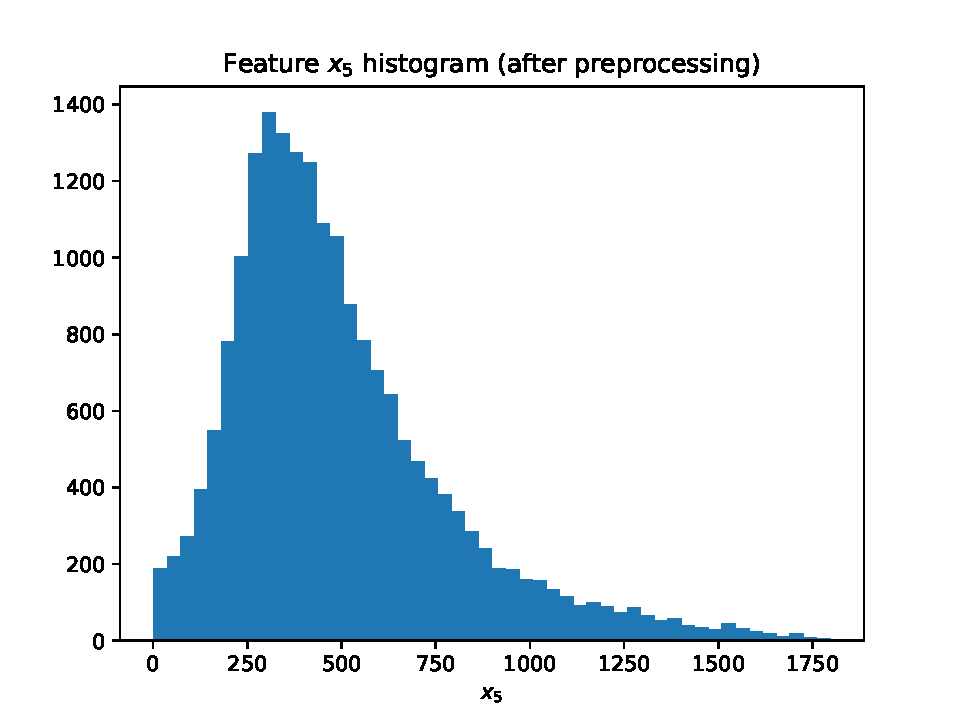
\includegraphics[width=.43\textwidth]{real_dataset_3/hist_feat_5_after.pdf}
  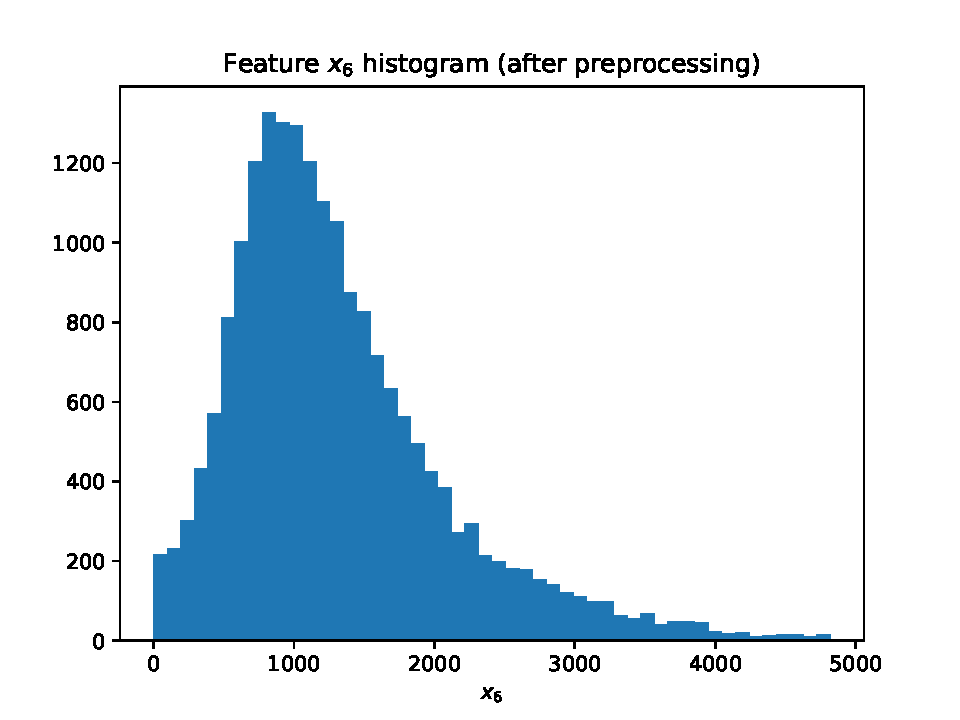
\includegraphics[width=.43\textwidth]{real_dataset_3/hist_feat_6_after.pdf}\\
  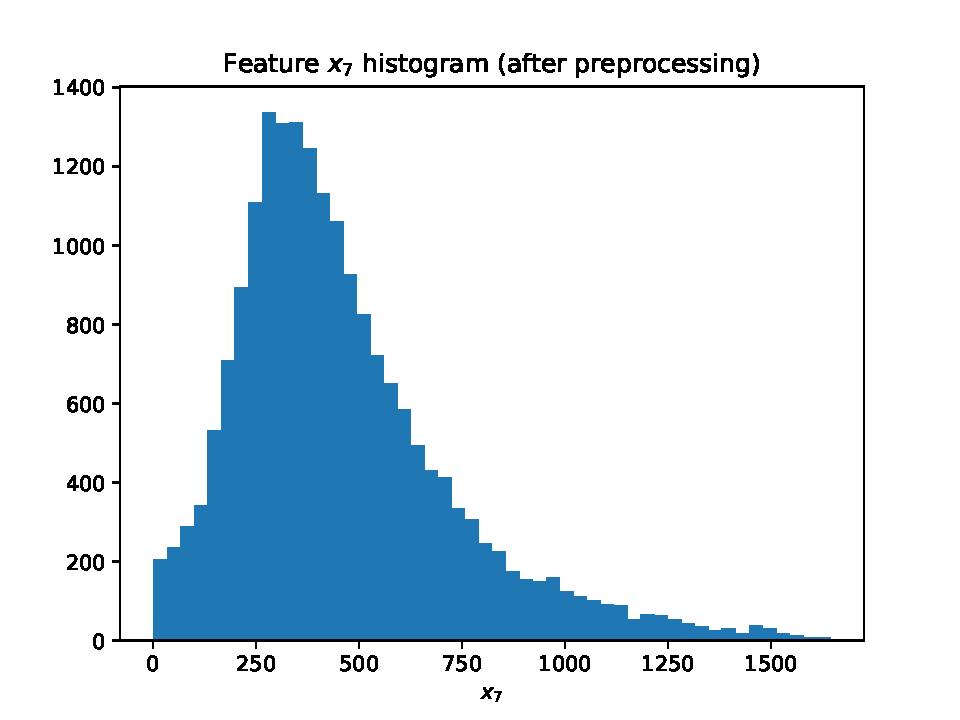
\includegraphics[width=.43\textwidth]{real_dataset_3/hist_feat_7_after.pdf}
  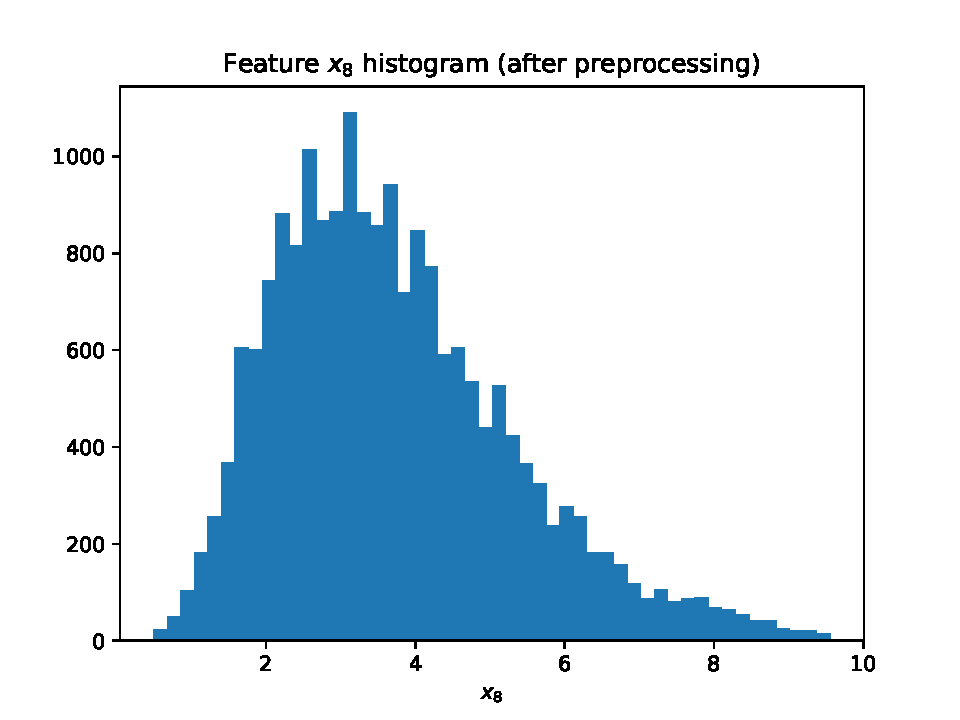
\includegraphics[width=.43\textwidth]{real_dataset_3/hist_feat_8_after.pdf}\\
  \label{fig:feature-histograms}
  \caption{The Histogram of each feature in the California Housing Dataset.}
\end{figure}



\begin{figure}[h]
  \centering
  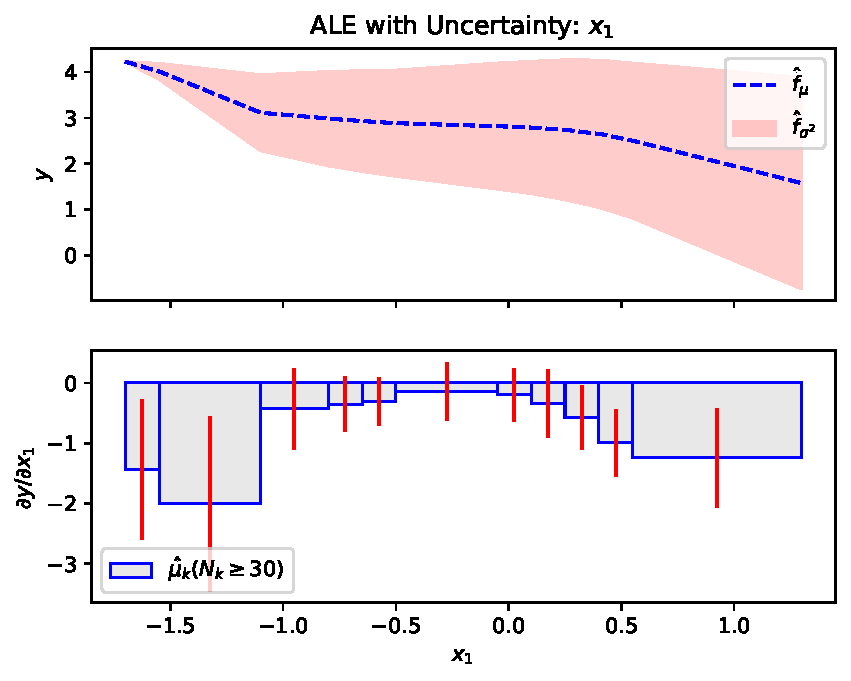
\includegraphics[width=.24\textwidth]{real_dataset_3/feature_0_ale_auto.pdf}
  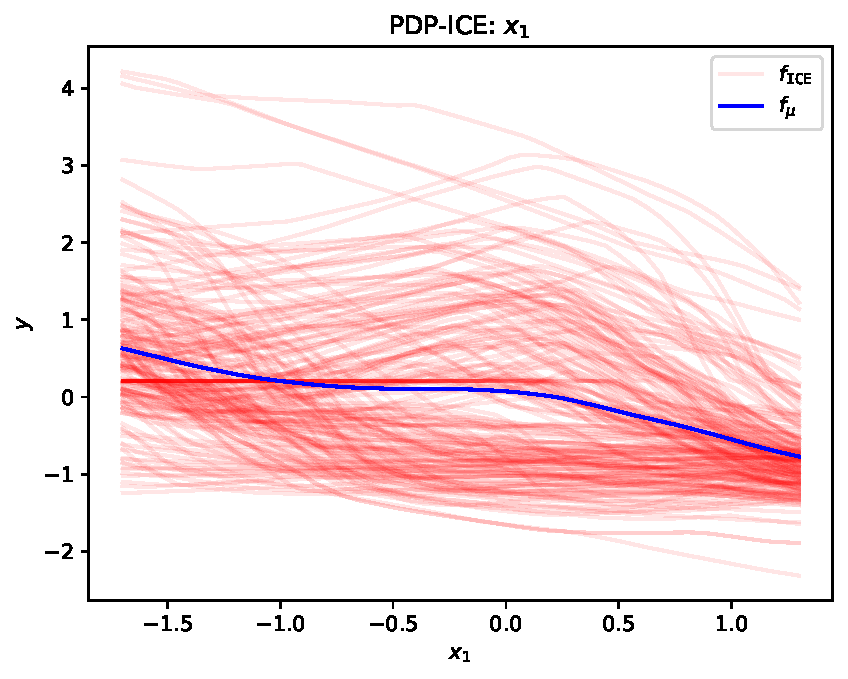
\includegraphics[width=.24\textwidth]{real_dataset_3/feature_0_pdp_ice.pdf}
  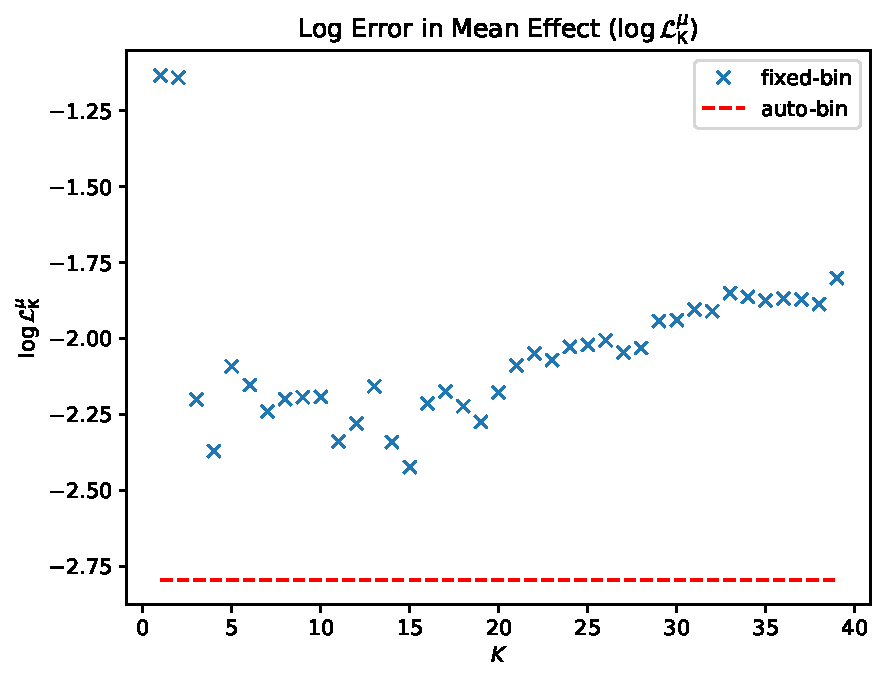
\includegraphics[width=.24\textwidth]{real_dataset_3/compare_mu_err_feature_0.pdf}
  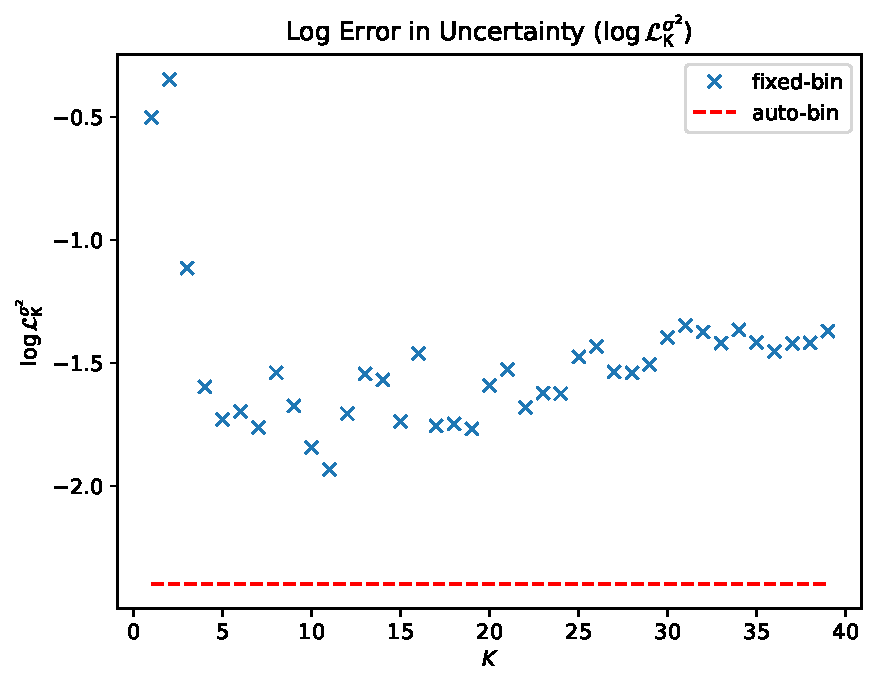
\includegraphics[width=.24\textwidth]{real_dataset_3/compare_var_err_feature_0.pdf}\\
  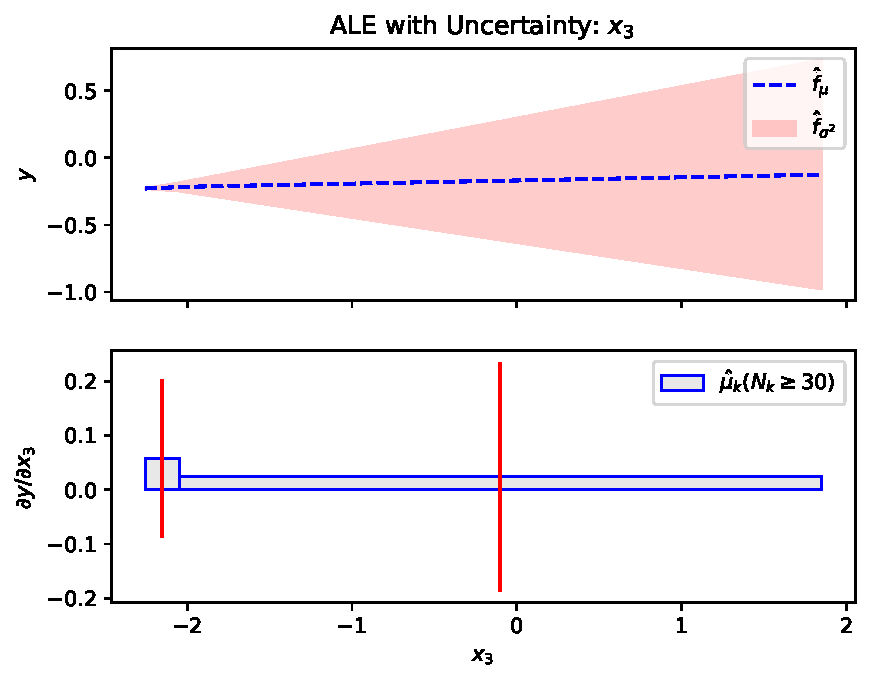
\includegraphics[width=.24\textwidth]{real_dataset_3/feature_2_ale_auto.pdf}
  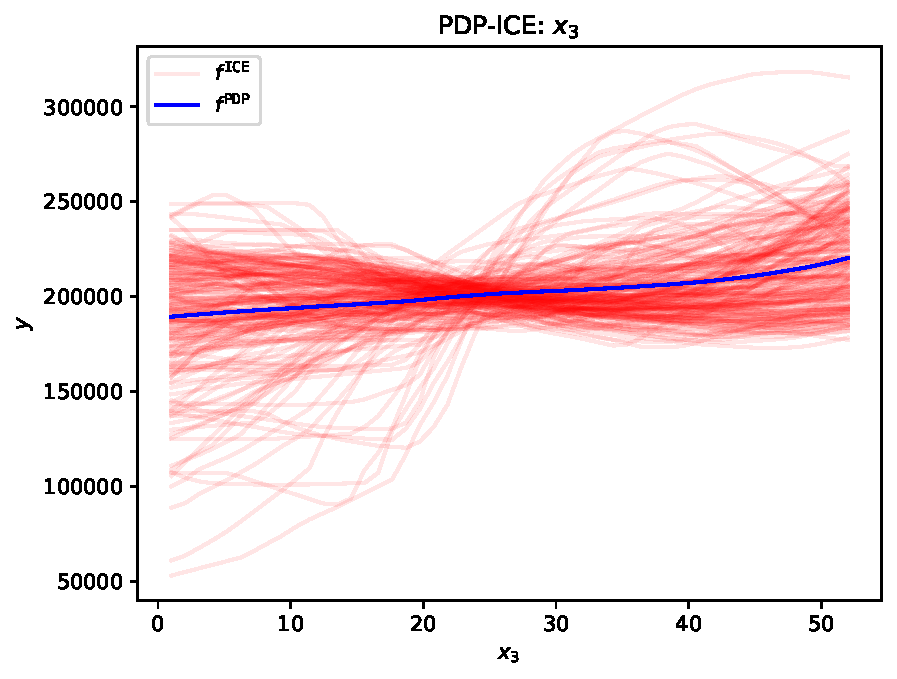
\includegraphics[width=.24\textwidth]{real_dataset_3/feature_2_pdp_ice.pdf}
  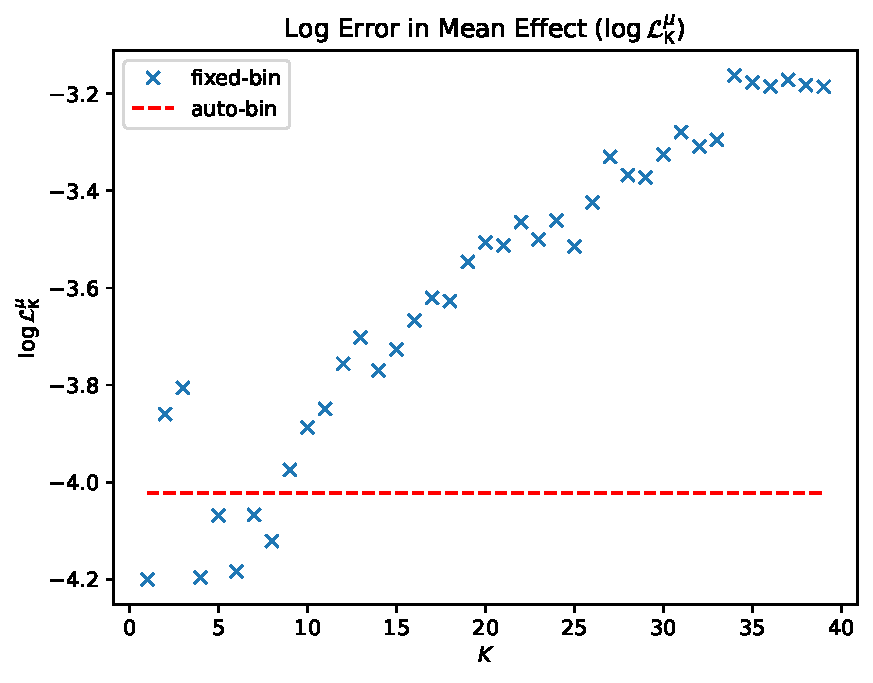
\includegraphics[width=.24\textwidth]{real_dataset_3/compare_mu_err_feature_2.pdf}
  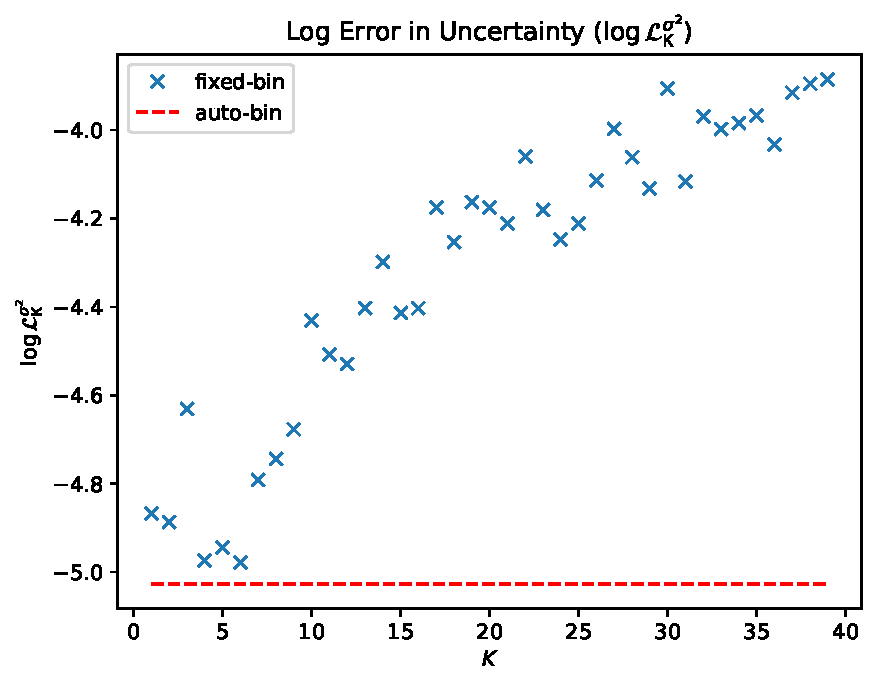
\includegraphics[width=.24\textwidth]{real_dataset_3/compare_var_err_feature_2.pdf}\\
  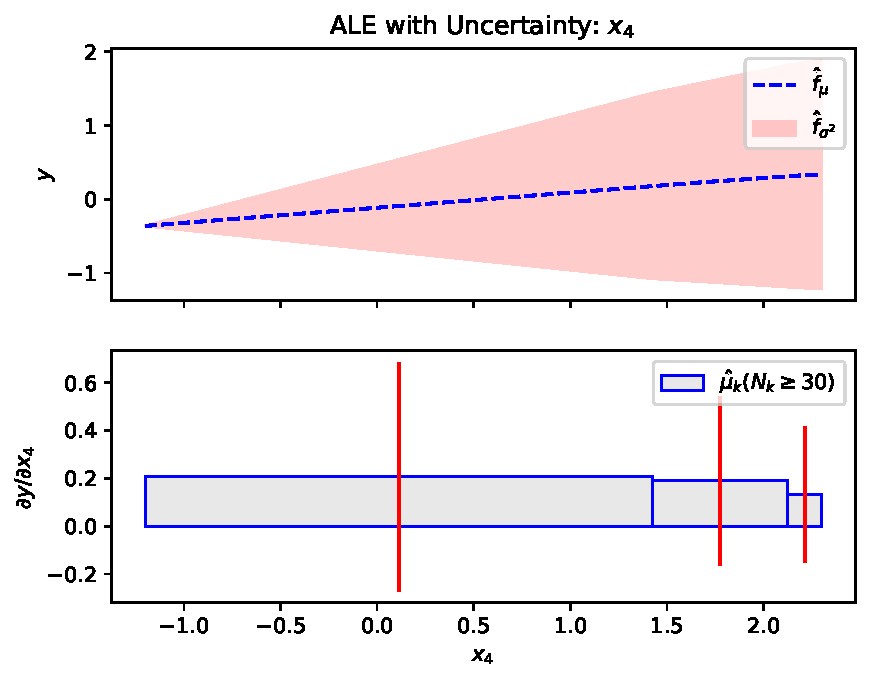
\includegraphics[width=.24\textwidth]{real_dataset_3/feature_3_ale_auto.pdf}
  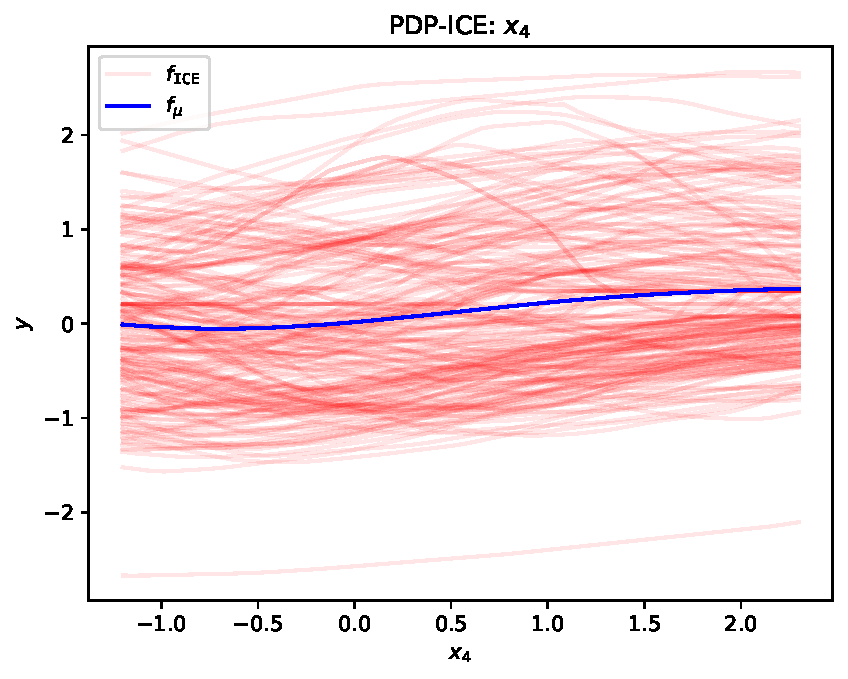
\includegraphics[width=.24\textwidth]{real_dataset_3/feature_3_pdp_ice.pdf}
  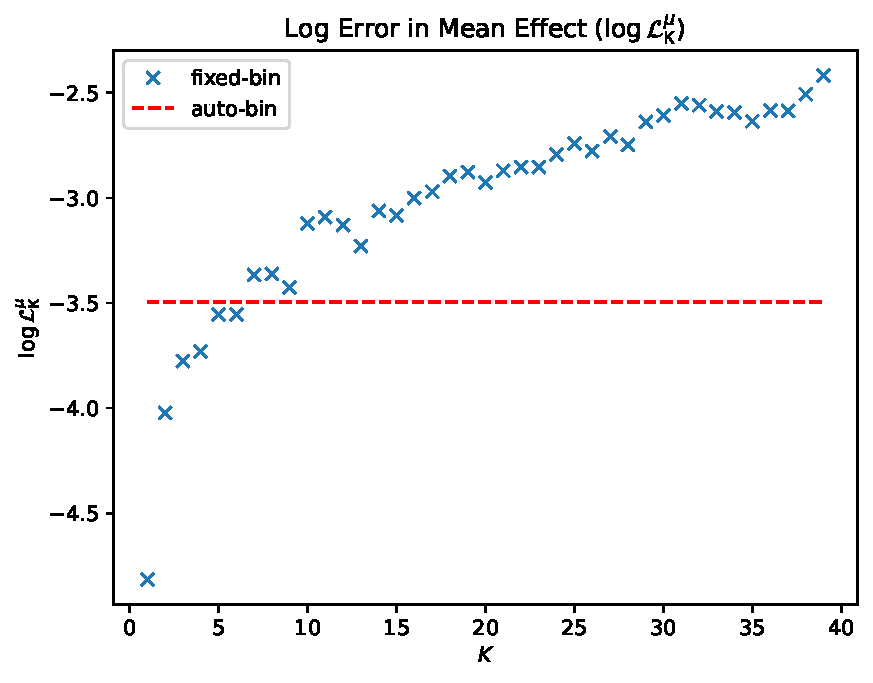
\includegraphics[width=.24\textwidth]{real_dataset_3/compare_mu_err_feature_3.pdf}
  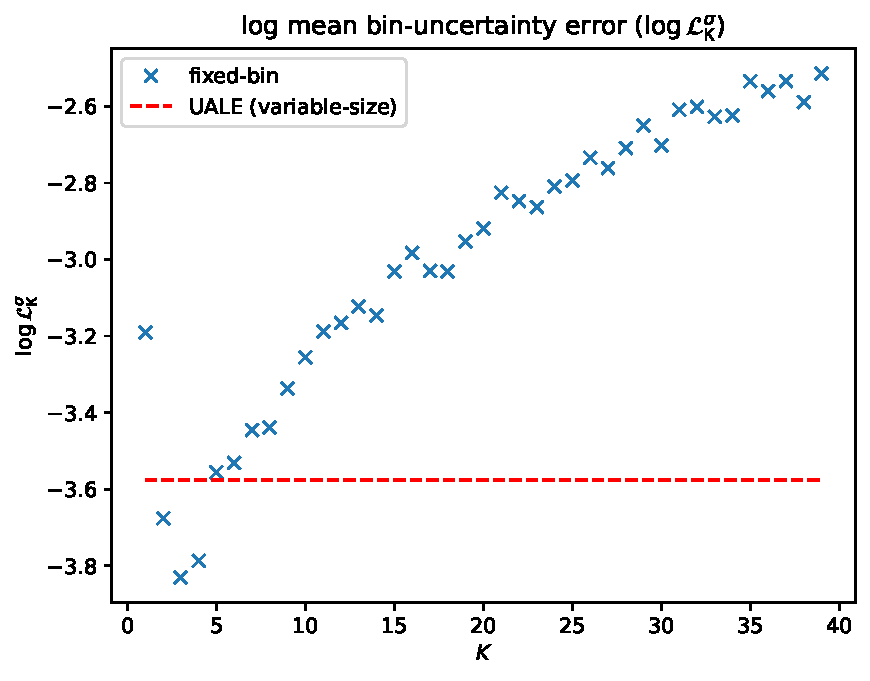
\includegraphics[width=.24\textwidth]{real_dataset_3/compare_var_err_feature_3.pdf}\\
  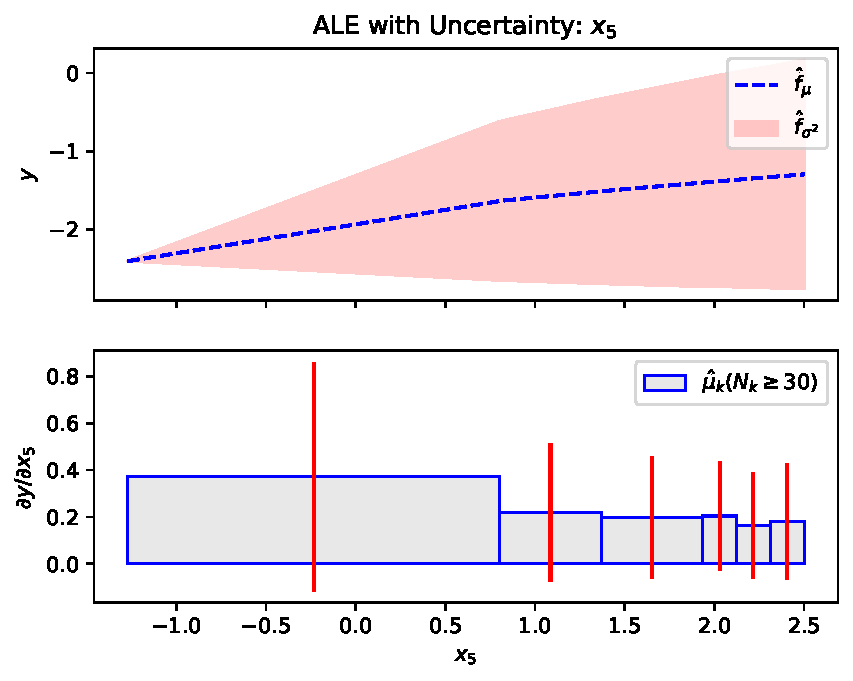
\includegraphics[width=.24\textwidth]{real_dataset_3/feature_4_ale_auto.pdf}
  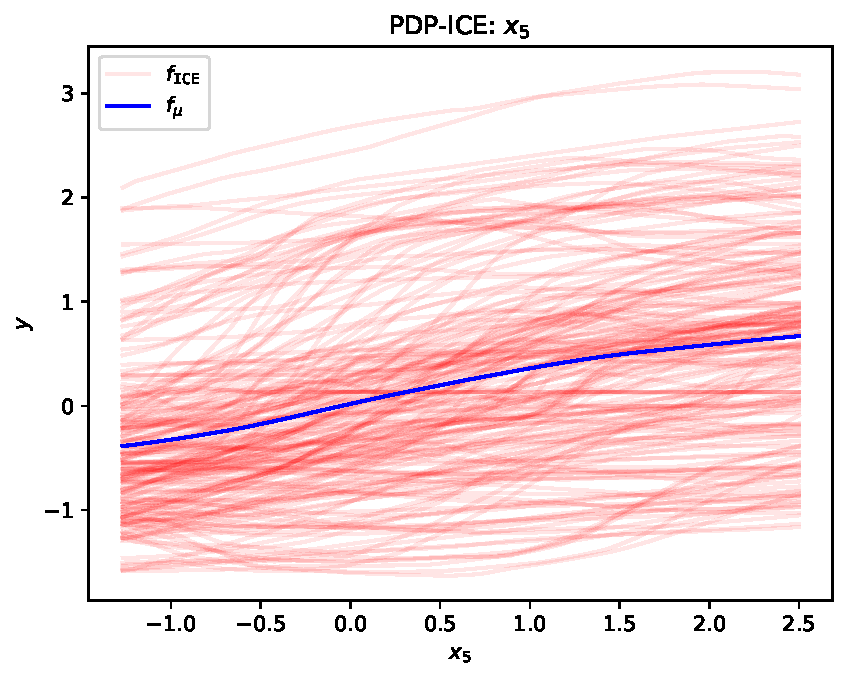
\includegraphics[width=.24\textwidth]{real_dataset_3/feature_4_pdp_ice.pdf}
  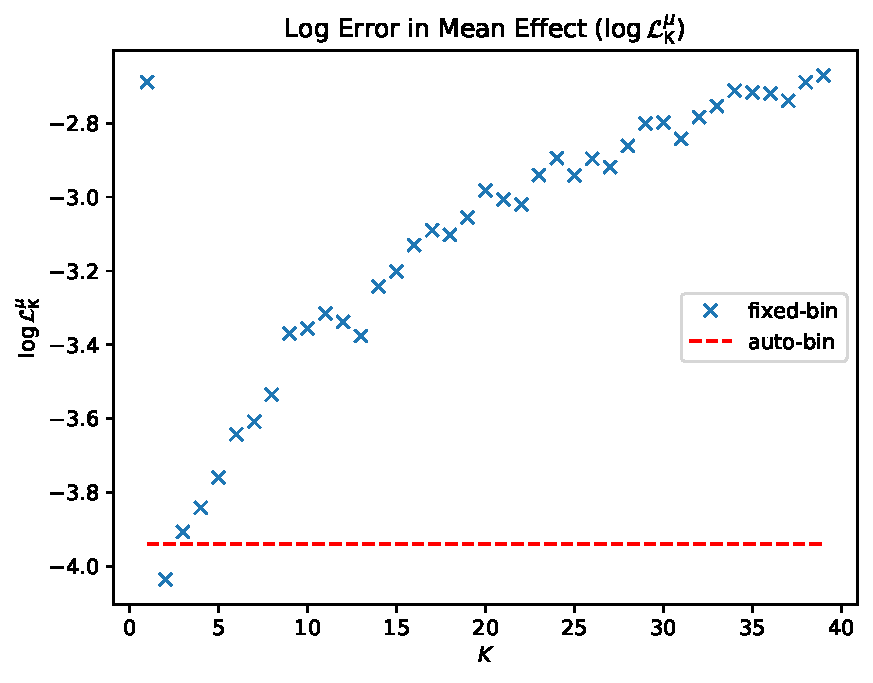
\includegraphics[width=.24\textwidth]{real_dataset_3/compare_mu_err_feature_4.pdf}
  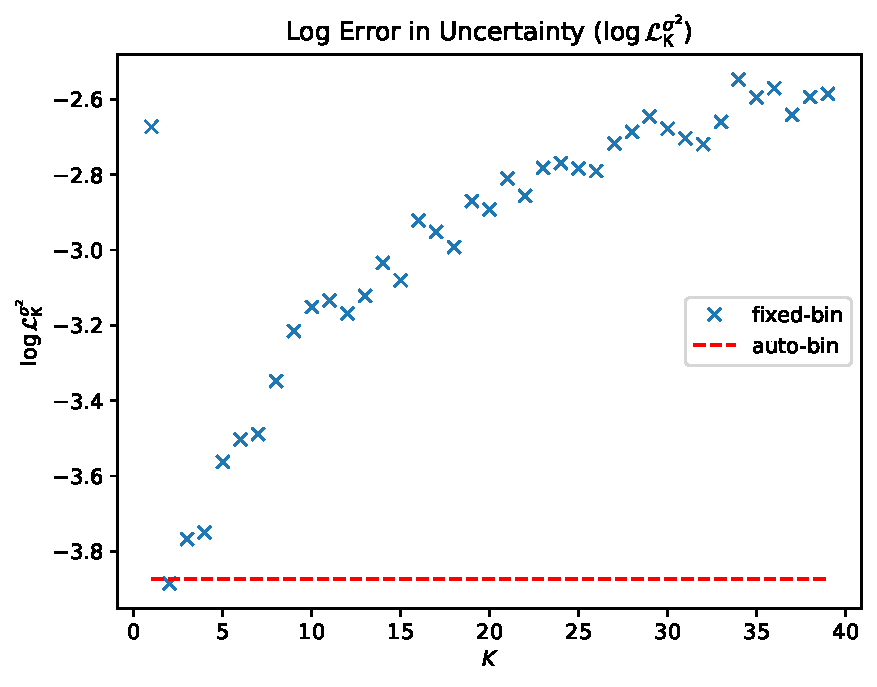
\includegraphics[width=.24\textwidth]{real_dataset_3/compare_var_err_feature_4.pdf}\\
  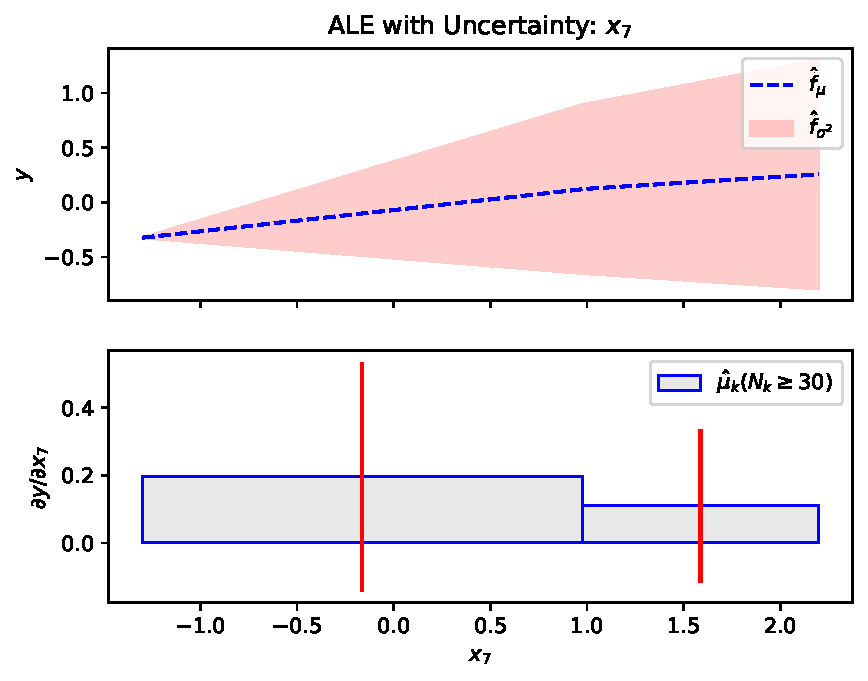
\includegraphics[width=.24\textwidth]{real_dataset_3/feature_6_ale_auto.pdf}
  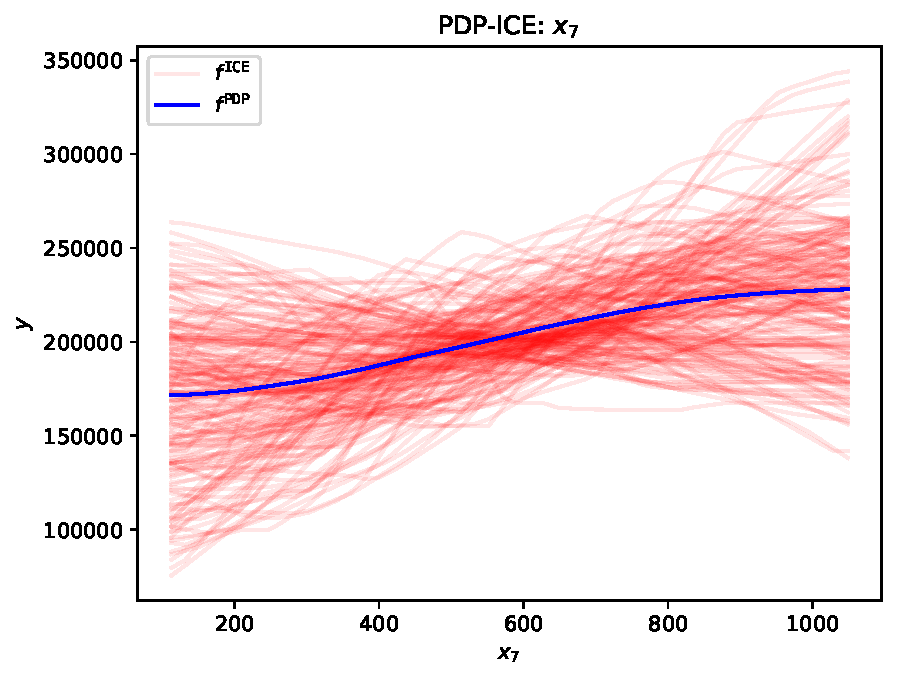
\includegraphics[width=.24\textwidth]{real_dataset_3/feature_6_pdp_ice.pdf}
  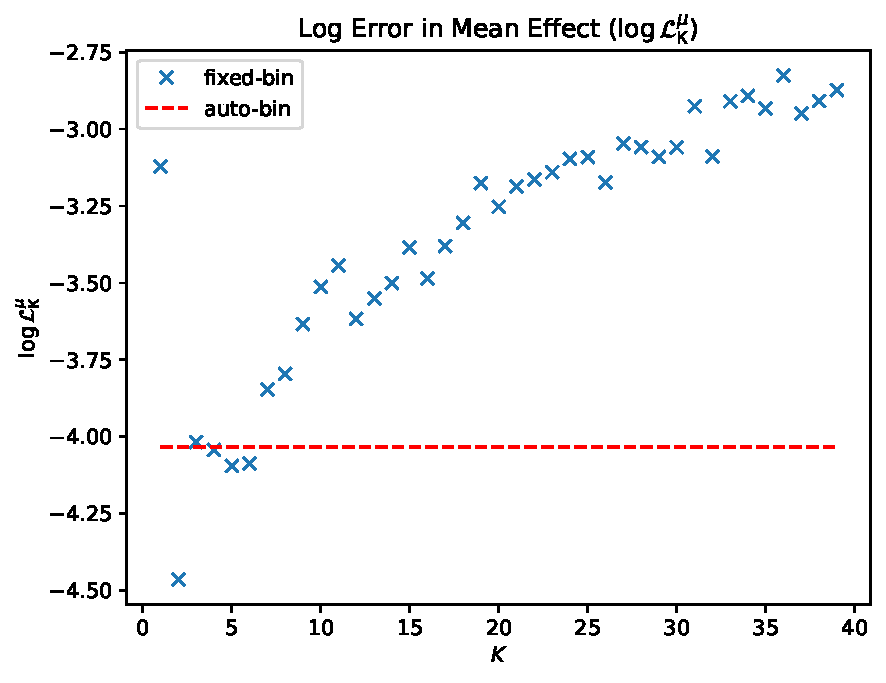
\includegraphics[width=.24\textwidth]{real_dataset_3/compare_mu_err_feature_6.pdf}
  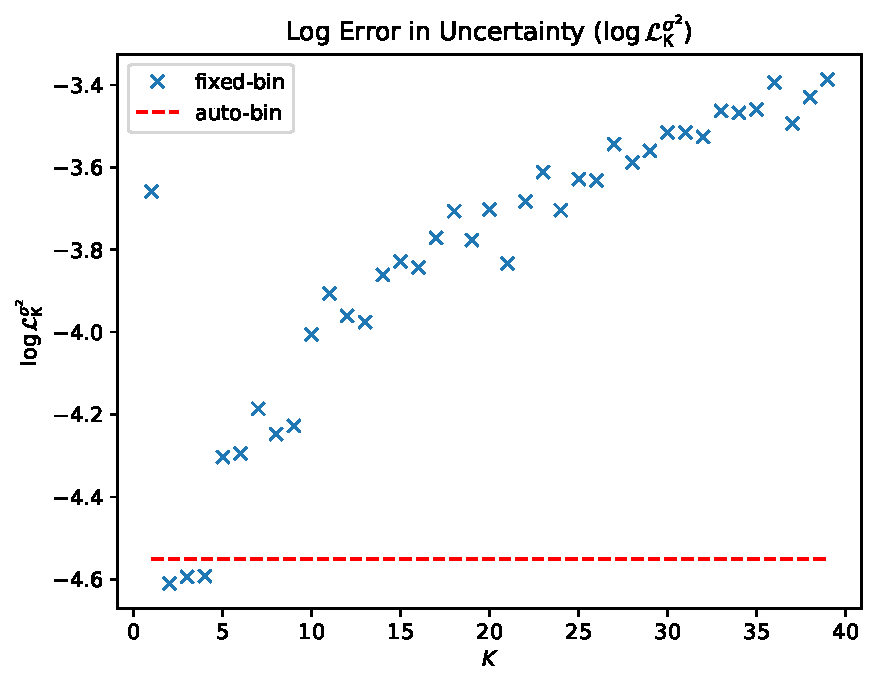
\includegraphics[width=.24\textwidth]{real_dataset_3/compare_var_err_feature_6.pdf}\\
  \caption{From left to right: (a) UALE plot, (b) PDP-ICE plot, (c) UALE vs fixed-size \(\mathcal{L}^{\mu}\) and (d) UALE vs fixed-size \(\mathcal{L}^{\sigma}\). From top to bottom, features \(x_1, x_3, x_4, x_5, x_7, x_8\).}
  \label{fig:ex-real-1}
\end{figure}


% \section{Further Experimentation}


% \section{MISSING PROOFS}

% The supplementary materials may contain detailed proofs of the results that are missing in the main paper.

% % \subsection{Proof of Lemma 3}

% % \textit{In this section, we present the detailed proof of Lemma 3 and then [ ... ]}


% % Given that,

% % The mean effect at a specific point \(x_s\) is:

% % \begin{equation}
% %   \label{eq:3}
% %   \mu(x_s) = \mathbb{E}_{\xc|x_s}\left [\dfdx (x_s, \xc) \right ]
% % \end{equation}


% % The variance at a specific point \(x_s\) is:

% % \begin{equation}
% %   \label{eq:3}
% %   \sigma^2(x_s) = \mathrm{Var}_{\xc|x_s}\left [\dfdx (x_s, \xc) \right ]
% % \end{equation}


% % The mean effect inside the interval \([z_1, z_2)\) is:

% % \begin{equation}
% %   \label{eq:1}
% %   \mu(z_1, z_2) = \frac{1}{z_2-z_1} \int_{z_1}^{z_2} \mathbb{E}_{\xc|x_s}\left [\dfdx (x_s, \xc)\right ]
% % \end{equation}

% % The accumulated variance inside the interval is:

% % \begin{equation}
% %   \label{eq:2}
% %   \sigma^2(z_1, z_2) = \int_{z_1}^{z_2} \mathbb{E}_{\xc|x_s=z} \left [ \left ( \frac{\partial f}{\partial x_s}(x_s, \xc) - \mu(z_1, z_2) \right )^2 \right] \partial z
% % \end{equation}


% % The residual at a specific point \(x_s\) is:

% % \begin{equation}
% %   \label{eq:4}
% %   \rho(x_s) = \mu(x_s) - \mu(z_1, z_2)
% % \end{equation}


% % We want to prove that:

% % \begin{equation}
% %   \label{eq:5}
% %   \sigma^2(z_1, z_2) = \int_{z_1}^{z_2} \sigma^2(z) + \rho^2(z) \partial z
% %   = \int_{z_1}^{z_2} \sigma^2(z) + \int_{z_1}^{z_2} \rho^2(z) \partial z
% % \end{equation}

% % Proof:


% % \begin{gather}
% %   \sigma^2(z_1, z_2) = \int_{z_1}^{z_2} \mathbb{E}_{\xc|x_s=z} \left [ \left( \frac{\partial f}{\partial x_s}( z, \xc) - \mu(z_1, z_2) \right)^2 \right] \partial z \\
% %   = \int_{z_1}^{z_2} \mathbb{E}_{\xc|x_s=z} \left [ \left ( \frac{\partial f}{\partial x_s} - \mu(z) + \rho(z) \right )^2 \right] \partial z \\
% %   = \int_{z_1}^{z_2} \left(
% %   \mathbb{E}_{\xc|x_s=z} \left [ (\frac{\partial f}{\partial x_s} - \mu(z) )^2 \right ]  +
% %   \mathbb{E}_{\xc|x_s=z} \left [ \rho(z)^2 \right] +
% %   \mathbb{E}_{\xc|x_s=z} \left [ 2(\frac{\partial f}{\partial x_s} - \mu(z) )\rho(z) \right ] \right )  \partial z \\
% %   = \int_{z_1}^{z_2}(\sigma^2(z) + \rho^2(z) + 2(\mu(z)-\mu(z))\rho(z))\partial z \\
% %   = \int_{z_1}^{z_2} \sigma^2(z)  + \rho^2(z) \partial z \\
% % \end{gather}


% \section{ADDITIONAL EXPERIMENTS}

% If you have additional experimental results, you may include them in the supplementary materials.

% \subsection{The Effect of Regularization Parameter}

% \textit{Our algorithm depends on the regularization parameter $\lambda$. Figure 1 below illustrates the effect of this parameter on the performance of our algorithm. As we can see, [ ... ]}

\vfill

\end{document}
